\subsection{Ejercicio de Parcial}

\begin{figure}[H]
\centering
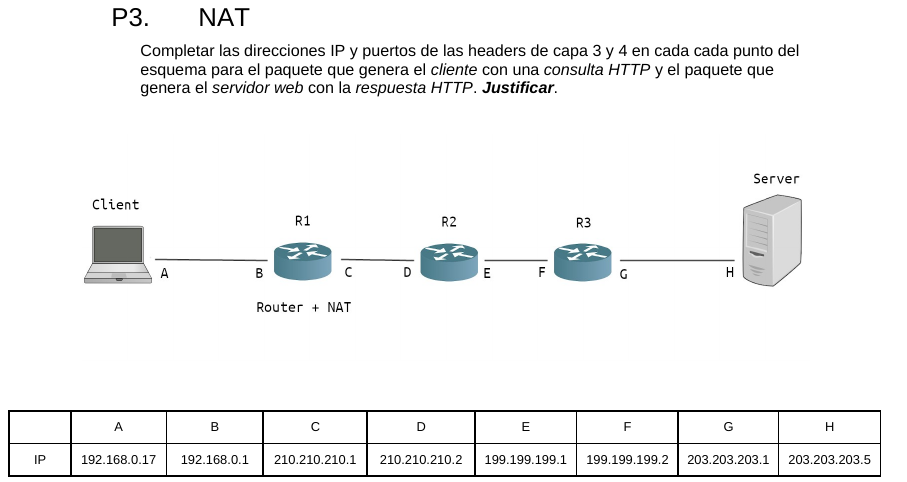
\includegraphics[width=\textwidth]{imagenes/enunciadoNat.png}
\end{figure}

\begin{table}[H]
    \centering
    \begin{tabular}{c|c|c|c|c}
         & IP origen & IP destino & Puerto Origen & Puerto Destino \\
         \hline
         \hline
        A & 192.168.0.17 & 203.203.203.5 & 3333 & 80 \\
        B &  192.168.0.17 & 203.203.203.5 & 3333 & 80\\
        C &  210.210.210.1 & 203.203.203.5 & 5001 & 80\\
        D &  210.210.210.1 & 203.203.203.5 & 5001 & 80\\
        E &  210.210.210.1 & 203.203.203.5 & 5001 & 80\\
        F &  210.210.210.1 & 203.203.203.5 & 5001 & 80\\
        G &  210.210.210.1 & 203.203.203.5 & 5001 & 80\\
        H &  210.210.210.1 & 203.203.203.5 & 5001 & 80\\
    \end{tabular}
    \caption{Http Request}
    \label{tab:my_label}
\end{table}

En el camino de ida (request) el paquete sale con origen ip del cliente y destino ip del servidor (junto con los puertos). Al llegar a C y pasar por el NAT, lo que se modifica es la ip de origen junto con su puerto, ya que a partir de ahora el origen se situará en la ip de R1 (correspondiente con C) y un puerto asociado hasta llegar en ese estado al servidor

\begin{table}[H]
    \centering
    \begin{tabular}{c|c|c|c|c}
         & IP origen & IP destino & Puerto Origen & Puerto Destino \\
         \hline
         \hline
        H & 203.203.203.5 & 210.210.210.1 & 80 & 5001 \\
        G &  203.203.203.5 & 210.210.210.1 & 80 & 5001 \\
        F &  203.203.203.5 & 210.210.210.1 & 80 & 5001 \\
        E &  203.203.203.5 & 210.210.210.1 & 80 & 5001 \\
        D &  203.203.203.5 & 210.210.210.1 & 80 & 5001 \\
        C &  203.203.203.5 & 210.210.210.1 & 80 & 5001 \\
        B &  203.203.203.5 & 192.168.0.17 & 80 & 3333 \\
        A &  203.203.203.5 & 192.168.0.17 & 80 & 3333\\
    \end{tabular}
    \caption{Http Response}
    \label{tab:my_label}
\end{table}

En el camino de vuelta o respuesta del servidor, la ip de destino será en un principio la de C (y la de origen el servidor). Al pasar R1, cambia la ip de destino al destinatario final y creador de la request, A.